\documentclass{report}


\usepackage{blindtext}
\usepackage{multicol}
\usepackage{amsmath}
\usepackage{blindtext}

\usepackage[spanish]{babel}

\usepackage{geometry}
\geometry{
 a4paper,
 total={170mm,257mm},
 left=20mm,
 top=20mm,
}

\renewcommand{\tablename}{Tabla}
\renewcommand{\partname}{Bloque}

\title{Exit-To}
\author{Rosalía Giménez}
\date{2024-07-25}




\usepackage{Sweave}
\begin{document}
\Sconcordance{concordance:Informe.tex:Informe.Rnw:1 26 1 1 0 57 1 1 11 2 1 1 45 1 4 %
33 1}


\maketitle

% Insertar la tabla de contenidos
\tableofcontents

\section*{Introducción}
\normalsize
\begin{multicols}{2}
En este informe se describe el diseño de un panel de soporte para la toma de decisiones educativas
y vocacionales. Está pensado para el momento en el que el estudiante y la persona orientadora
(servicio de orientación escolar, profesorado, familiares) repasan las opciones educativas
disponibles previamente a realizar la inscripción administrativa en una titulación académica
determinada.
Antecedentes.
En los últimos años, pese a la tendencia a la baja, en
España mantenemos una tasa de abandono escolar
temprano superior a la media de la Unión Europea.
Una de las medidas que podrían mitigar esta situación
sería la posibilidad de realizar una buena orientación
vocacional, que mantenga al estudiante con la
motivación suficiente en el camino hacia el éxito.
Actualmente, se dispone de muchos sistemas que ofrecen información estadística o vocacional
centrada en el autoconocimiento. Nuestra aportación sería ofrecer información estadística sobre el
nivel de bienestar subjetivo que se asocia con determinadas profesiones y regiones en España.
Se trata de acompañar el momento de la entrevista entre la persona orientadora y cada estudiante,
utilizando el panel para que conocer mejor la realidad socio-profesional a través de datos
estadísticos actualizados.
Además de la información sobre opciones académicas, se pone el énfasis en valorar el bienestar
subjetivo, frente al económico (retribución) y social (reputacional) que las distintas opciones
educativas pueden llegar a proporcionar.
Siendo su público objetivo principal personas en su adolescencia, el estilo de los gráficos debe ser
claro, fresco y sencillo sin por ello perder rigor en el valor de la información aportada. Con una
estética tipo “Comic”.
El rol del orientador es introductorio pero secundario, no se trata de un intermediario, ya que el
estudiante podrá entender la información por si mismo y consultar el panel de manera autónoma.
En un primer momento, el adolescente visualiza las opciones desde un ordenador junto con la
persona orientadora, pero con posterioridad podría acceder desde su propio dispositivo móvil o
tablet para reflexionar de manera individual sobre su decisión vocacional.
Para indagar en este aspecto necesitamos datos sobre nivel de estudios y bienestar cruzados.
Datos que hemos encontrado en el ESS Data Porta l (https://ess.sikt.no/en/?tab=overview)
\end{multicols}

\section*{Tabla}

\begin{figure}[h!]
\caption{Valores estadísticos de las principales variables del estudio}
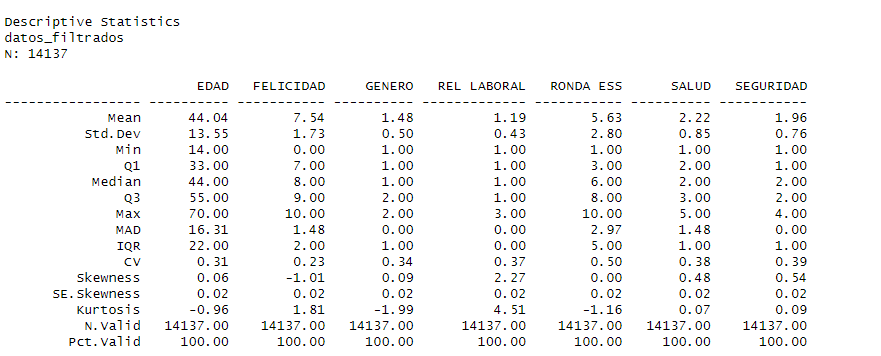
\includegraphics[scale=0.8]{DATOS_FILTRADOS.png}
\end{figure}




\section*{Gráfico}

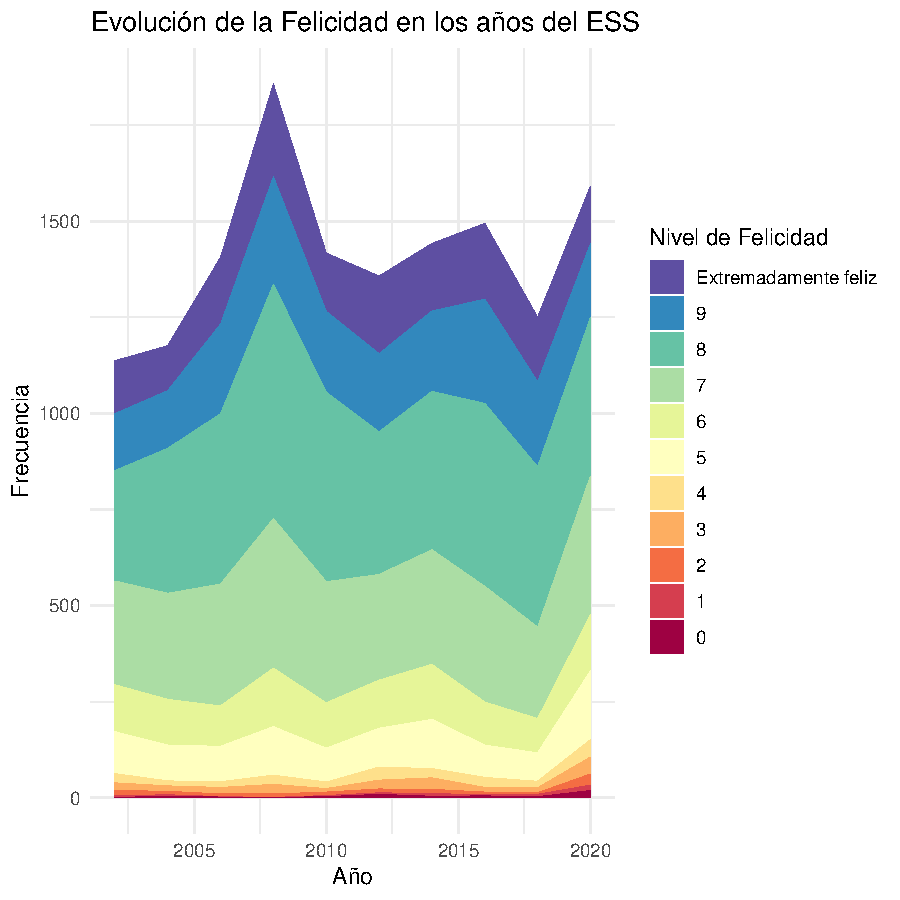
\includegraphics{Informe-grafico}


\section*{Conclusiones}

En este estudio, hemos dispuesto de una base de datos inicial de  19452. Eliminando los outliers el número se redujo a   14127 sujetos encuestados. Para poder cargar los datos en el Panel, tuvimos en cuenta solamente los datos con valores para el campo \emph{regiones}, siendo finalmente  5576 valores.

Al iniciar reto nos planteamos una serie de preguntas:

\begin{itemize}
\item \textbf{¿Quienes son los más felices? Los empleados, los autónomos o los que trabajan en un negocio
familiar? ¿Hay diferencias según el genero?}
\item ¿Cómo varían la felicidad, salud y seguridad en las diferentes regiones en los últimos años?
\item ¿En qué regiones viven las personas más infelices?
\item ¿Qué regiones presentan niveles más altos de personas que se sienten inseguras?
\item ¿Cómo podría afectar mi elección académica a mi calidad de vida y felicidad a largo plazo?
\item \textbf{¿Qué nivel de felicidad reportan las personas que han elegido un modelo determinado de relación
laboral?}
\item ¿Qué ocupaciones tienen las personas que se dicen felices? 
\item ¿Existen diferencias significativas en el nivel de felicidad reportado por hombres y mujeres en
función del modelo de relación laboral que han elegido?
\end{itemize}

Hemos encontrado algunas respuestas. 

\begin{enumerate}
\item En primer lugar, descubrimos que el nivel medio de felicidad es superior a 7 sobre 10 en general.
\item En segundo lugar, el tipo de relación laborarl no afecta significativamente al nivel de FELICIDAD, SALUD o SEGURIDAD, que en nuestro estudio consideramos como variables influyentes en el BIENESTAR SUBJETIVO.

\end{enumerate}

Los datos analizados revelan tendencias interesantes en la percepción de la felicidad a lo largo de los años. Este análisis puede ser utilizado para futuras investigaciones y políticas públicas.


%\section*{Tabla generada}

%\begin{table}[h!]
%\centering
%\caption{Valores estadísticos de las principales variables del estudio}


%<<tabla, echo=FALSE, results='asis'>>=
%library(xtable)
%xtable::xtable(datos_panel_Des)
%@

%\end{table}






\end{document}
